\cleardoublepage
\chapter{The Malleable Document}\label{ch:malleable}  % ``Aims \& objectives''?? Booooring

%\redmarginpar{This chapter needs to be rewritten. Will probably get to it once the other research chapters are mostly done}
%The real aim of this project is to produce documents that are adaptable to multiple viewing
%apertures, but do not require total reprocessing to do so.

%Chapter~\ref{ch:intro} goes into considerable detail
%about precisely which elements of a typeset document must be considered
%computation-heavy (and thus should be avoided if possible at view-time).
%This chapter goes some way towards defining exactly which portions of the
%typesetting process can be pre-computed and which cannot. It also analyses where shortcuts
%can be taken, and their effects on the final document.

\marginpar{The research in\\ this chapter was previously described in \cite{Pinkney2011}}

The invention of movable type in China in the 11th Century, and independently in Europe in the 15th Century, led to an enormous increase in the availability of printed material. In its various incarnations, movable type formed an extremely important part of the newspaper industry, from its advent in the 17th century, until digitisation in the mid-1980s.

The inherently volatile nature of newspaper layout (caused, for example, by important stories breaking shortly before going to press) coupled with the expense and time-consuming nature of physical typesetting, led to the development of the familiar columnar appearance of the newspaper that is prevalent worldwide.

\section{The use of Galleys in Typesetting}
\label{sec:galleys}
In a traditional newspaper layout, each page is divided into columns that are of equal width, or \gls{measure}. All text that is to appear in the newspaper is typeset to fit this measure (or integer multiples thereof, for example in the case of headlines) allowing articles to be slotted anywhere into the final layout of the newspaper, simply by breaking the article text between lines where necessary to span across columns or pages. An article never requires retypesetting as long as its content remains unchanged\ed{}an advantage only available when all text is rendered to fit into columns of the same width.


The metal trays used to contain typeset lines of physical type are known as \glspl{galley}. Newspapers use reasonably narrow galleys; paperback books tend to use wider galleys, and hardback books wider still. \marginpar{A brief survey of various items of print within arms' reach suggests that newspapers use approximately $2$'' galleys, paperback books around $4$'', and hardback books around $5$''. This thesis uses a galley width of $4\frac{2}{3}$''} Narrower galleys offer the advantage that less space is wasted if the final line in a paragraph does not span the full width: this is more important in newspaper layout than in most other typesetting situations, since space is at a premium. Wider galleys aid readability, up to a certain point, after which it becomes difficult for the eyes to keep track between lines \cite{Bringhurst2008, Braganza2009, Voorhees2011}.

Typographer Robert Bringhurst~\cite{Bringhurst2008} has stated that lines ranging in length between 45 and 75 characters (including both letters and space produces satisfactory layouts for a single-column page, and that the 66-character line is widely regarded as ideal. He has also asserted that an average of 40--50 characters is reasonable for multiple-column work. Furthermore, he has stated that line lengths exceeding 75--80 characters make continuous reading difficult, and that at the other end of the spectrum, lines shorter than 38--40 characters are unlikely to be easy to fully justify, and should therefore in most cases be set \gls{raggedright}.


Typesetting text into physical galleys is directly analogous to precomputing many of the `hard' parts of typesetting. In particular, all hyphenation, line breaking, \gls{justification}, \gls{kerning}, \gls{glyph} substitution, and so forth (in fact all horizontal layout) is `compiled out' as the galley is created.

When the galleys are later fitted to a physical page, there is no requirement to re-typeset any of the horizontal layout: only vertical layout problems remain, such as attempting to avoid widowed and orphaned lines (where the last/first lines of a paragraph appear first/last in a column) and choosing optimal placements of figures and other floating bodies. What remains is a problem similar to that described by Michael F. Plass in his Ph.D. thesis \cite{Plass1981}, and by Donald E. Knuth in Chapter~15 of The \TeX{}book~\cite{Knuth1984}.

\section{Galleys as a Reflow Tool}
\label{sec:singlegalleymetric}
As described in the previous section, setting the text of a document into a galley provides it with some limited flowability. Specifically, the document can be paginated to fit any page which is at least as wide as the galley, and of arbitrary height. Wider pages may be able to accommodate multiple columns, but unless the page size is chosen carefully, based on the galley's width, there is likely to be noticeable extra horizontal whitespace, particularly if the page width is not close to a multiple of the galley width.


\begin{figure}
 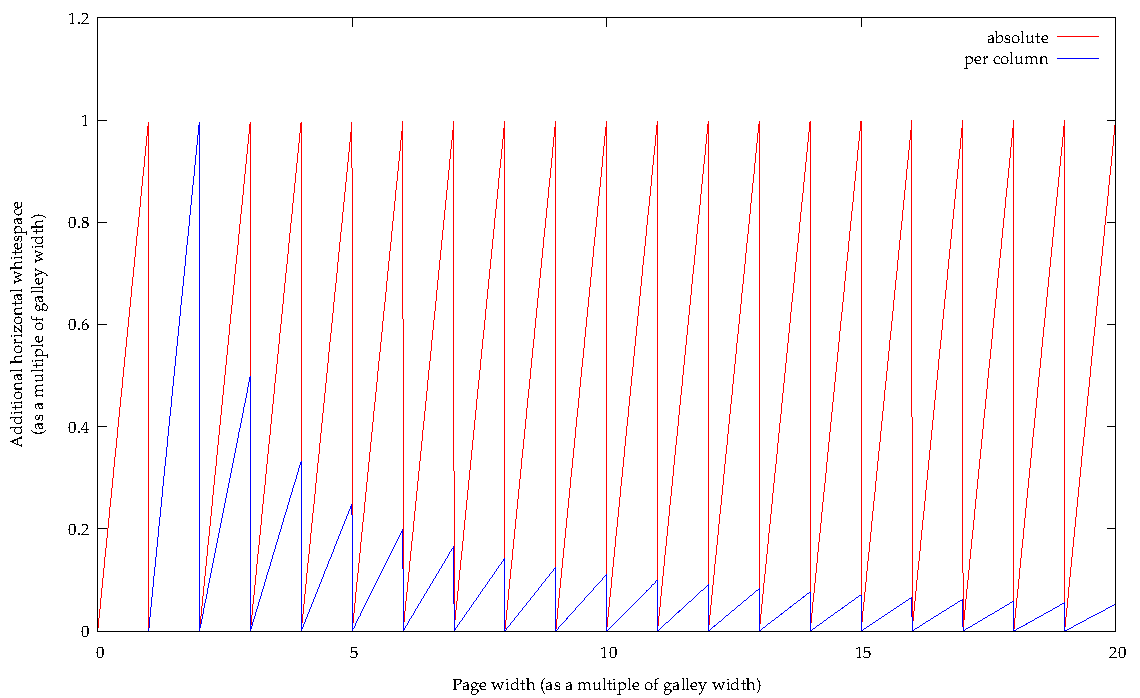
\includegraphics[height=\textwidth,angle=90]{gnuplot/1col}
 \caption[Extra whitespace in a single-galley document]{As more columns fit on a page, the extra whitespace required per column decreases}
 \label{fig:sawtooth}
\end{figure}


Figure~\ref{fig:sawtooth} shows how the extra horizontal whitespace on a page varies with page width. The peaks occur just before the point where an extra column can be added, and the amount of extra whitespace that is required drops to a minimum. The blue line shows the extra whitespace divided by the number of columns that fit on the page, which gives a more useful metric to work with: if we physically divide the extra whitespace and insert it between the columns to increase their spacing (as opposed to leaving it on the right- or left-hand margins) then the wider the page, the less detriment is caused by the extra fraction of galley width.

\emph{This process of setting text into galleys and reflowing can easily be simulated programatically, and it seems that this will be an effective way to pre-compute many of the more complex parts of the typesetting process, but without flowability being sacrificed.}

\section{Multiple Galley Renderings}
\label{sec:multigalleymetric}
The problem of extra whitespace can be overcome in several ways. Firstly, and most simply, the scaling of the galley could be altered, effectively simulating a change in the point size of the font. This is an obvious side-effect and is probably undesirable, unless a change in point size has explicitly been requested, and especially if the size change is particularly noticeable.

A second way in which columns can be better fitted to the page width is to typeset the source document into a range of galleys of varying \gls{measure}. When the document is to be rendered at view-time, the most appropriate measure (according to some metric) can be selected for display. One very simple metric is to select whichever galley rendering minimises the additional whitespace.

By overlaying the Figure \mbox{\ref{fig:sawtooth}-like} graphs for each galley, we are able to obtain a graph like Figure~\ref{fig:overlay}, which features all available galleys. If we use our simple metric of minimum whitespace, we can simply select whichever galley requires the smallest amount of extra whitespace for a given page width.

\begin{figure}
 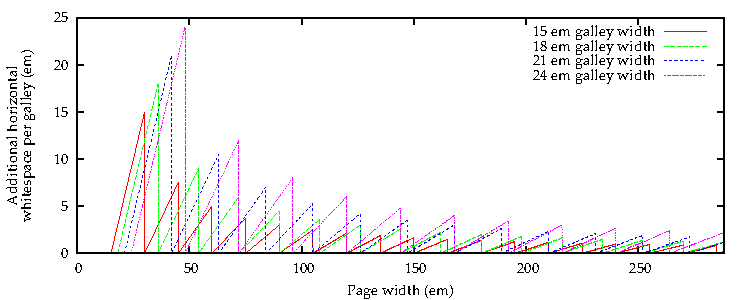
\includegraphics[height=\textwidth,angle=90]{gnuplot/overlay}
 \caption[Extra whitespace in a multi-galley document]{Overlaying the sawtooth graphs for several galleys of differing widths allows us to easily identify the galley that minimises extra added whitespace}
 \label{fig:overlay}
\end{figure}

\section{A Simple Implementation}
The algorithm described above was prototyped using existing tools from the University of Nottingham Document Engineering Laboratory: specifically, the \gls{cog} model \cite{Bagley2003} for creating and managing modularised \gls{pdf} documents. This was chosen specifically to avoid the need to write a typesetter or layout engine from scratch; typesetting is performed by the \troff{} suite, and the display of the final layout by Adobe Acrobat.  % though there is no reason why this algorithm could not be implemented with any other system capable of tightly specifying page imaging operations. Indeed, for this to be implemented in any non-prototypal form, \ie{} to be used on any portable device, it is likely that a specific, new rendering engine will need to be written for each device (or class of device).

\subsection{The \textsc{cog} Model}
%summary of cogs, what I've changed, ie line-level rather than default paragraph level. Put in tree to retain par details
The \gls{cog} model was developed to enable the reuse of semantic components within \pdf{} documents, by breaking the traditional graphically-monolithic \pdf{} page into a series of distinct, encapsulated graphical blocks, termed \glspl{cog}. Initial work on what later became the \gls{cog} model was conducted in the mid-1990s~\cite{Smith1995}, and further developed throughout the 2000s~\cite{Bagley2003,Bagley2004a,Bagley2005,Macdonald2005,Bagley2006,Bagley2007}. The \gls{cog} model, as described in the previous citations, does not account for any relationship between individual \glspl{cog}\,---\,it was simply designed as a method with which document components could be easily reused, reordered, or extracted. The \glspl{cog} generated are largely at the granularity of a paragraph, and still have no compunction to be imaged onto the page in any particular order (for example in reading order).

In order to implement a galley-based design, it was necessary to change the granularity at which the \glspl{cog} were produced, such that each line of text is represented by a separate \gls{cog}. However, it is also important that the semantic structure of the document is maintained. This is crucial for the process of layout at view-time: not only must the logical order of the document content be preserved, but also the relationship between each component of the content, such as which line belongs to which paragraph, whether a certain item is floatable, and so on.

The \gls{cog} model takes advantage of the fact that the \pdf{} specification \cite{Adobe2001} allows page content to be described by an array of streams of imaging operators, rather than the more commonly encountered single, monolithic stream. Unfortunately, this array is one-di\-men\-sional, meaning that whilst it can enforce reading order, it cannot be used, say, to group lines into paragraphs, or paragraphs into sections.

Since the \pdf{} specification allows essentially arbitrary \marginpar{According to the specification, \pdf{} readers that encounter unknown data within a \pdf{} file that they do not recognise should simply ignore it} insertion of data structures into a document, this flexibility was used to embed the document's structure as a tree, in parallel to the \pdf{}'s content array. The term \emph{Galley Structure Tree} will henceforth be used to refer to this data structure. (At this point, it is important to make the distinction between the term \emph{Galley Structure Tree} and the unrelated \emph{structure tree} that is defined in the \pdf{} specification and mentioned in Section~\ref{sec:fixedformats}.)

An example of a simple Galley Structure Tree is shown in Figure~\ref{fig:tree}. At the level of its leaves, this tree contains pointers to the \glspl{cog} which make up the content of the document. In the simplest case, where the document contains only one rendering (and thus the pa\-ra\-graph-level items have only one child) the \glspl{cog} pointed at by the leaves can simply be rendered in order, adding vertical space as appropriate.

\begin{figure}
 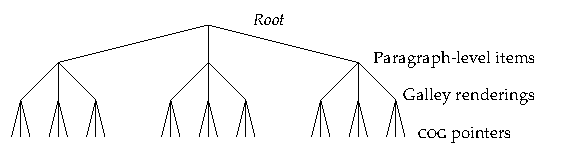
\includegraphics[width=\textwidth]{gfx/tree}
 \caption[A simple Galley Structure Tree]{A simple Galley Structure Tree. The first level below the root represents all paragraph-level items: headings, paragraphs, figures etc. These items have one child for each galley rendering of the document. These in turn have one child for each \gls{cog} comprising their content\ed{}in the case of a paragraph or heading its lines; in the case of a figure, the figure itself and any associated caption.}
 \label{fig:tree}
\end{figure}

\subsection{The Source Document}\label{sec:srcdoc}
Since the majority of available tools for producing \gls{cog}ged \glspl{pdf} rely on the typesetting package \ditroff{}~\cite{Kernighan1982}, it was decided to use this as the basis for the source document. \Ditroff{} is particularly amenable to many of the features required here\ed{}it is quite happy to have its page size set to large values\ed{}one sample document used a page length of 2000 inches (approximately 50 metres) with no complaints from \ditroff{}. (This is important, as it avoids \emph{ditroff} performing any pagination, which would cause \COG{} resources being spread across multiple pages in the resultant \pdf{} file, which in turn would cause difficulties accessing these resources from other pages.) An example of a source document is shown in Listings \ref{lst:troffsourcedoc1}~and~\ref{lst:troffsourcedoc2}.



\begin{lstlisting}[label=lst:troffsourcedoc1,captionpos=b,float,caption={[A sample troff source document, part 1]A sample troff source document. The actual document text is in a file named {\tt contents.inc} , and is imported multiple times with the {\tt .so} macro. After each import, the current line length is changed (using, for example, {\tt .nr LL 1.5i} to set the Line Length register to 1.5 inches). The {\tt \textbackslash X} commands are used to pass arbitrary data through the typesetter, and into the resultant ditroff intermediate code for later use. In this case, it is used to pass the column width (hence ``cWidth'') in points, so that this data can later be embedded within the final \pdf{} file.}]
.nr HM 0.5i
.nr FM 0.5i
.ds CH 
.\" Overwrites the Centre Header (suppresses page number)
.pl 2000i
.\" Make the page quite long to avoid troff doing any pagination
.nr PO 0
.\" set Page Offset (ie left margin) to zero
.ps 11
.vs 13
.nr PS 11
.nr VS 13
.\" Set point size to 11 and vertical spacing (leading) to 13
.\" Below, alter value of LL (line length) and include document
.\" content with the .so macro
.nr LL 1i
\X'cWidth:72'
.\" Line Length (ie galley width)
.so contents.inc
.nr LL 1.5i
\X'cWidth:108'
.so contents.inc
.nr LL 2i
\X'cWidth:144'
.so contents.inc
.nr LL 2.5i
\X'cWidth:180'
.so contents.inc
.nr LL 3i
\X'cWidth:216'
.so contents.inc
.nr LL 3.5i
\X'cWidth:252'
.so contents.inc
.nr LL 4i
\X'cWidth:288'
.so contents.inc
\end{lstlisting}


\begin{lstlisting}[label=lst:troffsourcedoc2,captionpos=b,float,caption={[A sample troff source document, part 2]A three-paragraph excerpt from a sample {\tt contents.inc} file, as described in Listing~\ref{lst:troffsourcedoc1}. Each paragraph is preceded by a call of the {\tt.PP} macro, which signifies the start of a new paragraph.}]
.PP
Lorem ipsum dolor sit amet, consectetur adipiscing elit. Cras vel
enim vitae mauris vestibulum egestas. Suspendisse potenti.
Pellentesque leo nunc, lobortis vitae gravida vel, congue at
nulla. Praesent a placerat mauris. Praesent sed erat ac dui
tincidunt consectetur vel nec leo. In velit odio, congue non
eleifend at, accumsan eu diam. Suspendisse dignissim, quam quis
euismod laoreet, est leo euismod lectus, sed consequat leo nunc
in ante. Duis risus tellus, suscipit ut fermentum et, ornare non
lorem. Morbi nibh elit, dignissim ullamcorper posuere at, lacinia
condimentum odio. Fusce vitae metus mi. Pellentesque scelerisque
fermentum magna a dictum. Mauris ut ante mauris, ac viverra
felis. Praesent ut elit ut purus malesuada suscipit. Fusce mollis
eros ac lectus suscipit gravida. Pellentesque vel nisl nec eros
convallis luctus nec eu quam. Aliquam tincidunt ultrices blandit.
.PP
Vestibulum lorem felis, consectetur ornare vehicula ac, cursus
tincidunt nisl. Aliquam in enim nisi, quis hendrerit est. Nullam
pretium congue sapien ac tincidunt. Suspendisse suscipit felis
eget nibh luctus sit amet imperdiet ligula venenatis. Vestibulum
eu dui nulla. Vivamus interdum ullamcorper sapien eget dapibus.
Proin sed dictum arcu. Curabitur velit justo, fringilla non
sodales laoreet, dignissim nec nulla. Praesent convallis ipsum
quis dolor ultricies non sodales dui viverra. Phasellus nec nisi
at nisi bibendum aliquam vitae et arcu. Donec feugiat dolor ut
felis dapibus eget auctor enim mattis.
.PP
Curabitur eget eros neque, in pulvinar massa. Suspendisse ac
massa quis justo fringilla consectetur. Vivamus lacinia tincidunt
purus, sit amet ullamcorper neque imperdiet quis. Nulla at lectus
turpis, in semper augue. Donec eu rhoncus turpis. Maecenas lectus
lacus, porta et dictum eget, eleifend a nibh. Vestibulum pulvinar
pellentesque lectus, et tincidunt eros consequat sed. Duis risus
lorem, placerat et molestie ut, porta a mi. Fusce eu elit enim,
id consequat nibh. Cras elementum, odio a tristique rutrum, nibh
neque sodales lorem, eu feugiat ipsum leo a nunc. Quisque enim
felis, luctus dapibus iaculis ac, tempor vitae lacus. Nunc eu mi
quis lacus scelerisque tincidunt. Sed sed nulla dui. Suspendisse
porta imperdiet tortor vel ultricies. Donec sit amet ligula
velit. Nulla tempor, risus sit amet congue aliquam, est nulla
tincidunt lectus, scelerisque cursus lacus diam vel metus. Donec
eu elit dolor. Nullam id libero ac metus ornare iaculis id ut
lorem. Quisque iaculis justo nec nibh interdum vuPPutate.
\end{lstlisting}

\subsection{pdfdit}
\label{sec:pdfdit}

The output from \ditroff{}, Ditroff Intermediate Code, is very expressive, and, unlike \TeX's equivalent \textsc{dvi}, contains enough information that post-processors are easily able to locate the start and end of lines and paragraphs within the document. This meant that only minimal changes were needed to the \emph{pdfdit} package,~\cite{Bagley2003} which was developed to produce \gls{cog}-\pdf{} from \troff{} documents.

The first modification necessary was to alter the granularity of the output \gls{cog}s, to produce them at line level, rather than at paragraph level. Secondly, some method of generating the requisite tree representing the document structure was required. Fortunately, since \emph{pdfdit} could already detect paragraphs, this code was adapted to create a new node in the Galley Structure Tree. Each subsequent line-level \gls{cog} produced can then be added as a child of this node.

The general algorithm for the processes alluded to in Sections \ref{sec:srcdoc} and~\ref{sec:pdfdit} is detailed below:
\begin{enumerate}
\item The \troff{} document's line length is set to a small value (2 inches or less) in order to produce a narrow column of text, and its page length to a very large value, to prevent pagination.
\item Following this, the actual document content is inserted several times, and the line length increased after each iteration, producing one document effectively containing multiple galley-width renderings of the same content.
\item The source document is then processed with \ditroff{} to generate the Ditroff Intermediate Code.
\item The Ditroff Intermediate Code is processed by \emph{pdfdit} to produce a \gls{cog} representation of the document, then it amalgamates the tree representations of each of the various galley widths into a Galley Structure Tree, in the form indicated in Figure~\ref{fig:tree}.
\item Finally the \pdf{} file is serialised, replete with \gls{cog}s and Galley Structure Tree.
\end{enumerate}


Various key excerpts from a malleable \pdf{} file's internal structure are shown in Listings \ref{lst:pdfstart}, \ref{lst:pdfpartree}, \ref{lst:pdfcog}, and~\ref{lst:pdfpages}

\begin{lstlisting}[label=lst:pdfstart,captionpos=b,language=postscript,float,caption={[Excerpt from a malleable document \pdf{}]An excerpt from a the start of a malleable document \pdf{} file. A reference to the \texttt{/ParagraphData} object (shown in Listing~\ref{lst:pdfpartree}) has been added to the \pdf{}'s \texttt{/Catalog} object. The \texttt{/Pages} object is also shown\ed{}note that there is only ever one page in a malleable \pdf{}.}]
%PDF-1.4
1 0 obj
<<
 /Type /Catalog
 /Pages 2 0 R
 /CogData 7472 0 R
 /ParagraphData 7473 0 R
>>
endobj
2 0 obj
<<
 /Type /Pages
 /Kids [7471 0 R  ]
 /Count 1
>>
endobj
\end{lstlisting}


\begin{lstlisting}[label=lst:pdfpartree,captionpos=b,language=postscript,float,caption={[Excerpt from a Galley Structure Tree]An excerpt from a Galley Structure Tree in a malleable document \pdf{} file. The tree structure described in Figure~\ref{fig:tree} can be observed in the \texttt{/Paragraphs} array, with the exception that the first element is an array containing the widths of each included galley rendering.}]
7473 0 obj
<<
 /Type /Multi-Width
 /Paragraphs
 [
    [72 108 144 180 216 252 288] % Width of each set of paragraphs, in points (ie 72*inch)
    [ % Paragraph 1
        [4 0 R 6 0 R 8 0 R 10 0 R 12 0 R 14 0 R 16 0 R 18 0 R 20 0 R 22 0 R 24 0 R 26 0 R 28 0 R 30 0 R 32 0 R 34 0 R 36 0 R 38 0 R 40 0 R 42 0 R 44 0 R 46 0 R 48 0 R 50 0 R 52 0 R 54 0 R 56 0 R 58 0 R 60 0 R 62 0 R 64 0 R 66 0 R 68 0 R 70 0 R 72 0 R 74 0 R 76 0 R 78 0 R 80 0 R 82 0 R 84 0 R 86 0 R 88 0 R 90 0 R 92 0 R 94 0 R 96 0 R 98 0 R 100 0 R 102 0 R 104 0 R 106 0 R 108 0 R 110 0 R 112 0 R 114 0 R 116 0 R 118 0 R 120 0 R 122 0 R 124 0 R 126 0 R 128 0 R 130 0 R 132 0 R 134 0 R]
        [2303 0 R 2305 0 R 2307 0 R 2309 0 R 2311 0 R 2313 0 R 2315 0 R 2317 0 R 2319 0 R 2321 0 R 2323 0 R 2325 0 R 2327 0 R 2329 0 R 2331 0 R 2333 0 R 2335 0 R 2337 0 R 2339 0 R 2341 0 R 2343 0 R 2345 0 R 2347 0 R 2349 0 R 2351 0 R 2353 0 R 2355 0 R 2357 0 R 2359 0 R 2361 0 R 2363 0 R 2365 0 R 2367 0 R 2369 0 R 2371 0 R 2373 0 R 2375 0 R 2377 0 R 2379 0 R 2381 0 R 2383 0 R]
        [3755 0 R 3757 0 R 3759 0 R 3761 0 R 3763 0 R 3765 0 R 3767 0 R 3769 0 R 3771 0 R 3773 0 R 3775 0 R 3777 0 R 3779 0 R 3781 0 R 3783 0 R 3785 0 R 3787 0 R 3789 0 R 3791 0 R 3793 0 R 3795 0 R 3797 0 R 3799 0 R 3801 0 R 3803 0 R 3805 0 R 3807 0 R 3809 0 R 3811 0 R 3813 0 R]
        [4821 0 R 4823 0 R 4825 0 R 4827 0 R 4829 0 R 4831 0 R 4833 0 R 4835 0 R 4837 0 R 4839 0 R 4841 0 R 4843 0 R 4845 0 R 4847 0 R 4849 0 R 4851 0 R 4853 0 R 4855 0 R 4857 0 R 4859 0 R 4861 0 R 4863 0 R 4865 0 R 4867 0 R]
        [5661 0 R 5663 0 R 5665 0 R 5667 0 R 5669 0 R 5671 0 R 5673 0 R 5675 0 R 5677 0 R 5679 0 R 5681 0 R 5683 0 R 5685 0 R 5687 0 R 5689 0 R 5691 0 R 5693 0 R 5695 0 R 5697 0 R 5699 0 R]
        [6355 0 R 6357 0 R 6359 0 R 6361 0 R 6363 0 R 6365 0 R 6367 0 R 6369 0 R 6371 0 R 6373 0 R 6375 0 R 6377 0 R 6379 0 R 6381 0 R 6383 0 R 6385 0 R]
        [6951 0 R 6953 0 R 6955 0 R 6957 0 R 6959 0 R 6961 0 R 6963 0 R 6965 0 R 6967 0 R 6969 0 R 6971 0 R 6973 0 R 6975 0 R 6977 0 R 6979 0 R]
    ] % Note: "<x> <y> R" is a pointer to the object defined with "<x> <y> obj" -- these all point to COG spacer objects
    [ % Paragraph 2
        [136 0 R 138 0 R 140 0 R 142 0 R 144 0 R 146 0 R 148 0 R 150 0 R 152 0 R 154 0 R 156 0 R 158 0 R 160 0 R
%%% truncated %%%
\end{lstlisting}

\begin{lstlisting}[label=lst:pdfcog,captionpos=b,language=postscript,float,caption={[A \textsc{cog} and its associated spacer object]A \gls{cog} (object 2303) and its associated spacer (object 2304) from a malleable \pdf{}. The \gls{cog} object is never modified. To reposition the \gls{cog} on the page, the spacer object is deleted and replaced with a new one that has the required \texttt{/X} and \texttt{/Y} values set.}]
2303 0 obj
    <<
        /Type /XObject
        /Subtype /Form
        /Name /Cog8f692dee-5919-11e0-90bd-9eb109602c3e
        /FormType 1
        /BBox [0.000000 0.000000 82.933000 9.889000  ]
        /Baseline 2.387000
        /Indent 25.000000
        /Length 219
        /Resources <<
            /Font <<
                /R 3 0 R
            >>
            /ProcSet [/PDF /Text  ]
        >>
    >>
    stream
        q
        0.125000 0 0 0.125000 0 0 cm
        BT
        /R 1 Tf
        88.000000 0 0 88.000000 0.000000 19.096000 Tm (Lorem ) Tj
        88.000000 0 0 88.000000 448.000000 19.096000 Tm (i) Tj
        88.000000 0 0 88.000000 473.000000 19.096000 Tm (psum ) Tj
        ET
        Q
    endstream
endobj

2304 0 obj
    <<
        /Type /CogReference
        /Height 9.889000
        /Length 83
        /ptrTo /Cog8f692dee-5919-11e0-90bd-9eb109602c3e
        /X 25.000000
        /Width 82.933000
        /Y -14118.497000
    >>
    stream
        q 1 0 0 1 25.000000 -14118.497000 cm /Cog8f692dee-5919-11e0-90bd-9eb109602c3e Do Q 
    endstream
endobj
\end{lstlisting}


\begin{lstlisting}[label=lst:pdfpages,captionpos=b,language=postscript,float,caption={[Contents of a \pdf{} \texttt{Page} object]An excerpt from a malleable \pdf{} file showing that the \texttt{/Contents} of a \texttt{/Page} can be an array of content streams rather than one stream. In this case, each of the objects being pointed to are \gls{cog} spacers, as shown in Listing~\ref{lst:pdfcog}. Consequently, when a spacer object is deleted and a new one created (to reposition a \gls{cog} on the page) the \texttt{/Contents} array must be modified to reflect this.}]
7471 0 obj
<<
 /Type /Page
 /Subtype /Cogified
 /MediaBox [0 0 595 841]
 /Contents [5 0 R 7 0 R 9 0 R 11 0 R 13 0 R 15 0 R 17 0 R 19 0 R 21 0 R 23 0 R 25 0 R 27 0 R 29 0 R 31 0 R 33 0 R 35 0 R 37 0 R 39 0 R 41 0 R 43 0 R 45 0 R 47 0 R 49 0 R 51 0 R 53 0 R 55 0 R 57 0 R 59 0 R 61 0 R 63 0 R 65 0 R 67 0 R 69 0 R 71 0 R 73 0 R 75 0 R 77 0 R 79 0 R 81 0 R 83 0 R 85 0 R 87 0 R 89 0 R 91 0 R 93 0 R 95 0 R 97 0 R 99 0 R 101 0 R 103 0 R 105 0 R 107 0 R 109 0 R 111 0 R 113 0 R 115 0 R 117 0 R 119 0 R 121 0 R 123 0 R 125 0 R 127 0 R
%%% truncated %%%
\end{lstlisting}


\subsection{Acrobat Plugin}\label{sec:acroplugin}
\begin{figure}
 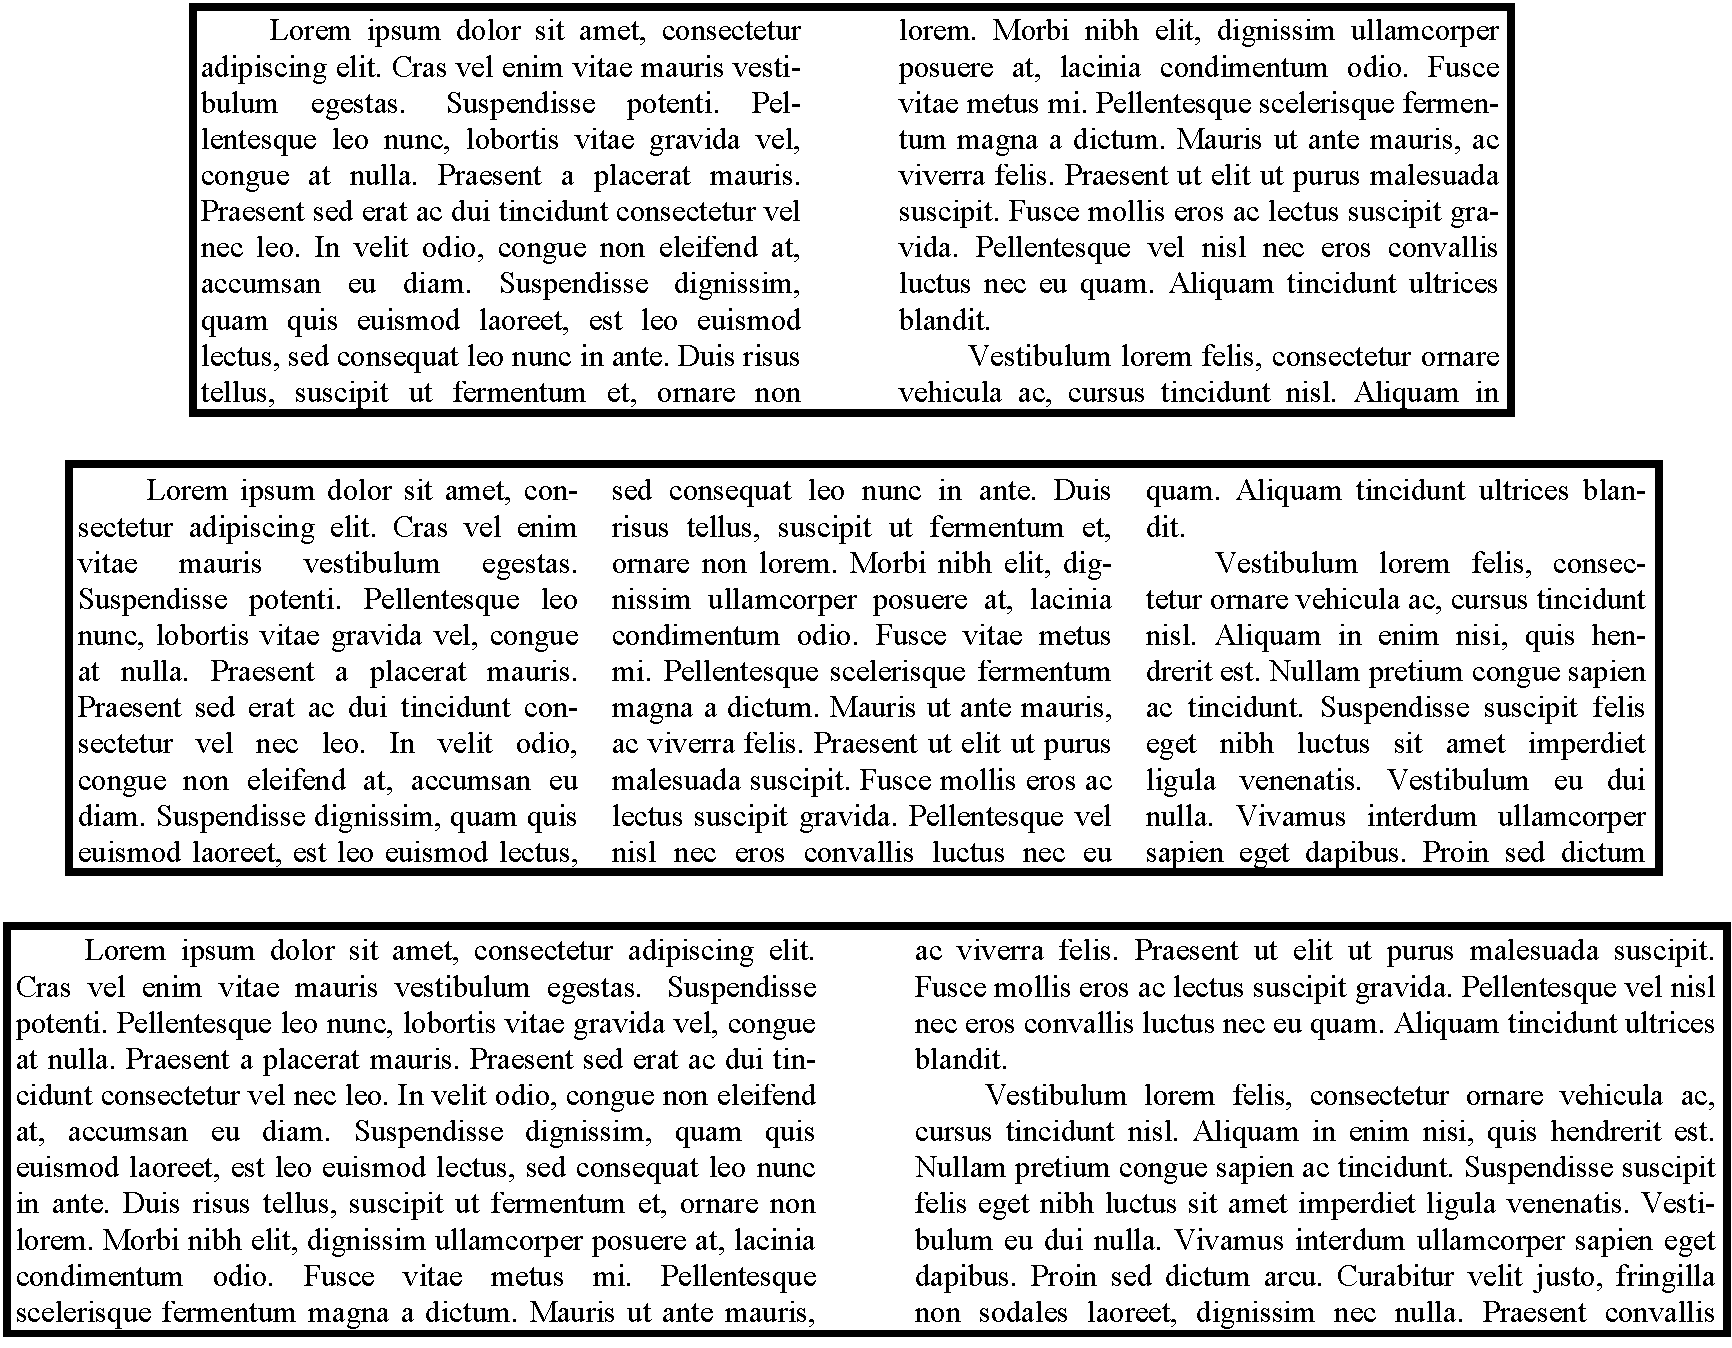
\includegraphics[width=\textwidth]{gfx/renderings-bbox}
 \caption[Sample renderings from the Acrobat plugin]{Three sample renderings from the Acrobat plugin, with page widths of 42, 48, and 54~em. Note that the middle rendering is considered to be a `better fit' than either the top or the bottom renderings, since the space between columns has been reduced, but that in each case, the galley rendering chosen is the one that minimises the space between columns for that particular page width.}
 \label{fig:renderings}
\end{figure}

The decision to use Acrobat as an `\ebook{} reader emulator' stemmed once again from the existing \gls{cog}-based tools (see Section \ref{sec:srcdoc}), as well as the extensive API and developer support available for Acrobat.

Since, by the point the document is to be displayed in Acrobat, most of the computationally expensive typesetting has already been carried out, the algorithm used to lay out the lines of the selected galley can be very simple.

The plugin chooses the most appropriate galley width to lay out, based on the current page width, and according to some measure of aesthetics (see both Section~\ref{sec:layout} and Chapter~\ref{ch:aesthetics}) and then simply lays the document out line by line, with appropriate vertical spacing, until no more lines will fit in the current column. Any subsequent columns which will fit on the same page are then laid out in the same manner.

For convenience of testing, the plugin also automatically resizes the page to that of the window of Acrobat, and re-lays out the text on the fly, allowing various combinations of page sizes, zoom levels, and aspect ratios to be trialled.
Some sample renderings from the Acrobat plugin are shown in Figure~\ref{fig:renderings}, and an excerpt of the code used for the layout is shown in Listing~\ref{lst:acrolayout}.

\begin{lstlisting}[language=c++,tabsize=4,basicstyle=\ttfamily\scriptsize\singlespacing,stringstyle=\color{blue},label=lst:acrolayout,captionpos=b,float,caption={[Acrobat plugin's layout algorithm]An excerpt from the C++ Acrobat plugin, showing the implementation of the layout algorithm described in Section~\ref{sec:acroplugin}.}]
int numPars = CosArrayLength(parArray) - 1; // first element is not a paragraph
CosObj widthsArray = CosArrayGet(parArray, 0); // it is the widths array
int numWidths = CosArrayLength(widthsArray);
ASFixed *widths = (ASFixed*)calloc(numWidths, sizeof(ASFixed));
double *badness = (double*)calloc(numWidths, sizeof(double));

int min_badness_index = 0;
int numCols = 0;

// Choose the "best" rendering
for (int i = 0; i < numWidths; i++) {
    widths[i] = CosFixedValue(CosArrayGet(widthsArray,i));
    int nc = pageWidth / (widths[i] + mingutter);
    ASFixed ex_ws = pageWidth % (widths[i] + mingutter);
    
    badness[i] = (ex_ws / 65536.0 + 100) * sqrt((double)nc);
    
    if (nc == 0) badness[i] = 1000 * i;
    
    if (badness[i] <= badness[min_badness_index]) {
        min_badness_index = i;
        numCols = nc;
    }
}

ASFixed colsep = pageWidth / numCols;
ASFixed linesep = 13<<16; // 13pt. (Ideally, infer from data within PDF)
ASFixed parsep = 0;

int curr_x = mediabox.left + (colsep - widths[min_badness_index]) / 2;
int curr_y = mediabox.top - topmargin;

CosObj newContents = CosNewArray(cosDoc, false, 100);

// Create new spacer objects with correct COGs, and insert into newContents
for (int p = 0; p < numPars; p++) {
    CosObj para = CosArrayGet(CosArrayGet(parArray, p + 1), min_badness_index);
    int numLines = CosArrayLength(para);
    for (int l = 0; l < numLines; l++) {
        CosObj baseline = CosDictGet(CosStreamDict(CosArrayGet(para, l)), ASAtomFromString("Baseline"));
        CosObj indent = CosDictGet(CosStreamDict(CosArrayGet(para, l)), ASAtomFromString("Indent"));
        CosObj name = CosDictGet(CosStreamDict(CosArrayGet(para, l)), ASAtomFromString("Name"));
        
        int y_offset = CosFixedValue(baseline);
        int x_offset = CosFixedValue(indent);
        
        if (curr_y < (mediabox.bottom + botmargin)) { //start new column
            curr_y = mediabox.top - topmargin;
            curr_x += colsep;
        }
        
        CCosDoc cDoc(cosDoc);
        CSpacerCreator spacerCreator(cDoc);
        CCosStream newSpacer = spacerCreator.Create(ASAtomGetString(CosNameValue(name)), curr_x + x_offset, curr_y - y_offset);
        
        CosArrayInsert(newContents, CosArrayLength(newContents), newSpacer);
        
        curr_y -= linesep;
    }
    curr_y -= parsep;
}

PDPageAddCosContents(page, newContents);


\end{lstlisting}


\section{Layout Considerations}
\label{sec:layout}
\begin{sidewaysfigure}
 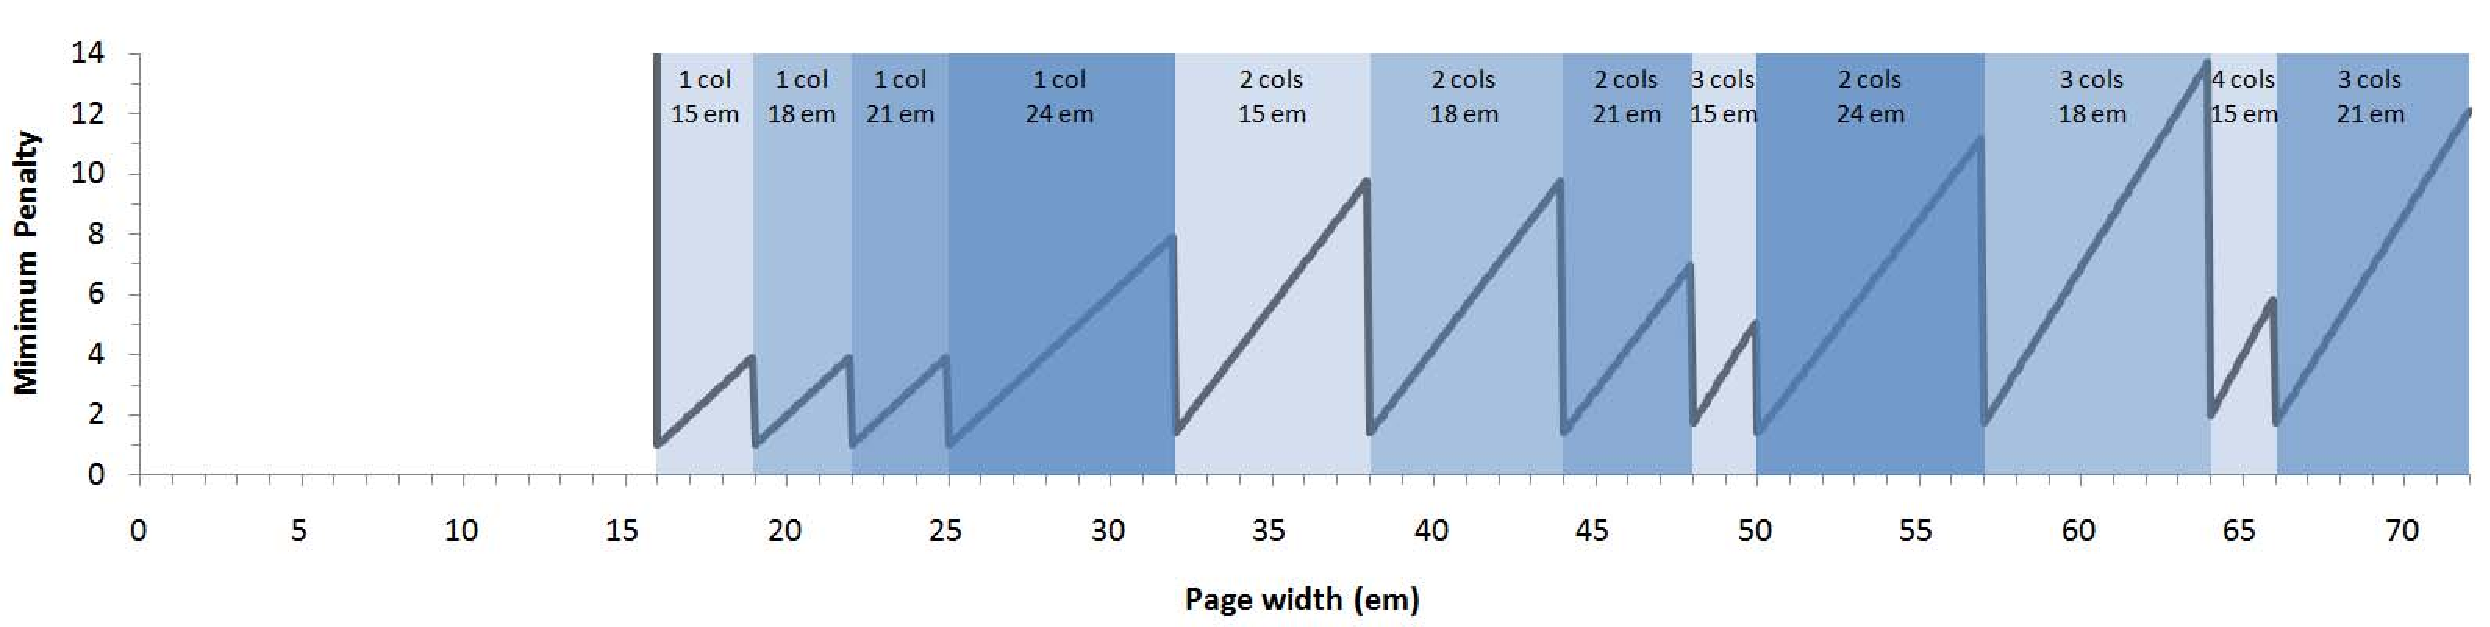
\includegraphics[width=\textwidth]{gfx/graph-em}
 \caption[Graph of minimum penalty values]{Graph showing the minimum penalty value of all galleys in a reflowable document, over a range of page widths. The particular document used contained four galleys; these were rendered at widths of 15, 18, 21 and 24~em, with a minimum gutter width of 1~em. Each vertical band highlights a range of page widths within which only the horizontal spacing of the page is altered. The boundaries between vertical bands represent a switch between galley renderings\ed{}the galley used and number of columns is as annotated on the graph.}
 \label{fig:penaltygraph}
\end{sidewaysfigure}

As discussed in Sections \ref{sec:galleys}, \ref{sec:singlegalleymetric}, and~\ref{sec:multigalleymetric}, galleys of text lend themselves to being used in a columnar format, and therefore a method of fitting columns appropriately to the available page width needed to be devised.

A sensible first approach is simply to calculate how many columns of each galley rendering will fit, by adding the galley width to a specified minimum inter-column spacing, and dividing the page width by the result. The remainder of this division will then specify the amount of additional horizontal whitespace required, which can then divided up and inserted between the columns.

A simple measure of aesthetic quality here is to apply a linear penalty for any extra whitespace required, as we seek to keep page margins and column gutters to a minimum.

Equations \ref{eqn:numcols} and~\ref{eqn:extraws} below show the formulae used to calculate the number of columns that will fit ($N_\text{cols}$), and the requisite extra whitespace ($S_\text{extra}$). $W_\text{page}$ is the total width of the page, $W_\text{galley}$ is the width of the current galley, and $W_\text{ICS}$ is the minimum required inter-column spacing.
\begin{equation}\label{eqn:numcols}
N_\text{cols}=\left\lfloor\frac{W_\text{page}}{W_\text{galley}+W_\text{ICS}}\right\rfloor
\end{equation}
\begin{equation}\label{eqn:extraws}
S_\text{extra}=W_\text{page}\!\!\mod \left(W_\text{galley}+W_\text{ICS}\right)
\end{equation}

As the page width increases, so must the widths of the inter-column gutters. In accordance with the extra-whitespace penalty, each galley rendering will produce penalties which vary in a sawtooth manner as the width of the page is increased. With a careful choice of galley widths, when these sawtooth penalties are overlaid, and the galley producing the minimum penalty chosen at each page width, a flatter and finer-toothed penalty graph emerges, as shown in Figure~\ref{fig:penaltygraph}.

In addition to penalising extra whitespace, wider columns should, in general, be favoured over narrower ones, i.e.~for a given page width, fewer, wider columns are generally considered preferable to a greater number of narrower columns. By multiplying the existing penalty by a smaller-than-linear function of the number of columns (experiments have been carried out with both logarithms and roots) the penalty may be subtly increased for greater numbers of columns.

The formula for the penalty used in Figure~\ref{fig:penaltygraph} is \begin{equation}P = (C + S_\text{extra})\cdot\sqrt{N_\text{cols}}\end{equation} where $P$ is the penalty, $S_\text{extra}$ is the extra whitespace required to be inserted (as computed in equation~\ref{eqn:extraws}), $N_\text{cols}$ is the number of columns which are required to fill the width of the page (as computed in equation~\ref{eqn:numcols}), and $C$ is a positive constant.

The purpose of the constant is to prevent the penalty from ever evaluating to zero, which would have the effect of disregarding the weighting of the number of columns. Figure~\ref{fig:penaltygraph} uses $C=1$.

This is calculated for each galley rendering, and the galley with the minimum value of $P$ is selected.
%eg what sort of layouts are we constricted to, and are they any good... cite Plass/Bringhurst

\section{Included galley renderings}
\label{sec:inc-renderings}
In order for a document to achieve optimal fit on every device of every conceivable size, we must produce one galley rendering of every conceivable width. Clearly, this is infeasible, both in terms of space and time. For reasons of practicality, we are therefore forced choose some finite subset of galley widths to include within a document.

Some experimentation has suggested that using between three and seven galley renderings, ranging in width between two and five inches (set in twelve point type) provides reasonable coverage on a variety of device sizes. Whether the sampling range within these bounds should be linear, or based on some other function, is still open for debate, and requires further experimentation.




\section{Efficiency}
%theoretically, how does it compare? Shove in lots of speculative Big Oh notation and try to sound authoritative. Or look at the algorithms used and actually be authoritative :)

It can easily be observed that the view-time complexity of the layout algorithm described in this chapter is linear.

At view-time, it must be decided which galley rendering to display: this is a trivial operation that requires one calculation per galley rendering. Assuming that there will never be more than ten galley renderings within one document (this seems reasonable given the discussion in Section~\ref{sec:inc-renderings}) the time taken to choose the best-fitting galley will always be dominated by the time taken to perform the layout itself.

Once the best-fitting galley rendering has been selected, all that is left is to traverse the Galley Structure Tree, laying out each line of text sequentially. When the bottom of the physical page is reached, text is then laid out in a new column adjacent to the previous one.

If there are $n$ lines of text in the document, this takes at most $k\cdot{}n$ operations, where $k$ is some constant pertaining to the operations required to lay out one line of text, and therefore the view-time complexity is $O(n)$.

A first-fit (or greedy) layout algorithm, as used by most current \ebook{} hardware and web browsers, also runs in $O(n)$, but proportional to the number of possible breakpoints rather than the number of lines of text. Due to using first-fit, the resultant layout will almost certainly be substandard in comparison to any high-quality pre-rendered layout, as used by the system described in this chapter. Conversely, to compute a higher-quality layout on the fly, (using, for example, the Knuth-Plass line breaking algorithm \cite{Knuth1981,Knuth1999}, or something even more complex) can take upwards of $O(n^2)$~\cite{Hirschberg1987,Eppstein1992,Hurst2009,Pinkney2013}.

\section{Summary}
The drawbacks of this system are that the filesize is necessarily increased (since data for multiple layouts must be included), and that the galley rendering that is displayed may not fit the available page width as snugly as an algorithm that has been run on the fly (which would therefore be specifically tailored to the dimensions of the page). In spite of this, this galley-based system produces pleasing-looking, well formatted documents.

The implementation of this algorithm within Adobe Acrobat is somewhat clunky\ed and certainly impractical to deploy on a real \ebook{} platform\ed but it demonstrates that the concept of pre-rendering several variants is a viable means to producing well-typeset flowable layouts.

The one notable omission from this chapter is support for floating blocks (such as figures)\ed only non-floating blocks are supported. In the next chapter, both of these issues are addressed.

